%%%%%%%%%%%%%%%%%%%%%%%%%%%%%% -*- Mode: Latex -*- %%%%%%%%%%%%%%%%%%%%%%%%%%%%
%% uhtest-body.tex -- 
%% Author          : Robert Brewer
%% Created On      : Fri Oct  2 16:30:37 1998
%% Last Modified By: Robert Brewer
%% Last Modified On: Mon Oct  5 16:01:29 1998
%% RCS: $Id: uhtest-body.tex,v 1.1 1998/10/06 02:07:14 rbrewer Exp $
%%%%%%%%%%%%%%%%%%%%%%%%%%%%%%%%%%%%%%%%%%%%%%%%%%%%%%%%%%%%%%%%%%%%%%%%%%%%%%%
%%   Copyright (C) 1998 Robert Brewer
%%%%%%%%%%%%%%%%%%%%%%%%%%%%%%%%%%%%%%%%%%%%%%%%%%%%%%%%%%%%%%%%%%%%%%%%%%%%%%%
%% 


\chapter{Introduction}

Every dissertation should have an introduction.  You might not realize
it, but the introduction should introduce the concepts, background,
and goals of the dissertation.

Examples of great literature can be found in table \ref{tab:example-1}.

%% Here is an example of how to create a floating table. Note that the caption
%% occurs _before_ the table, unlike a figure where it appears after!
%%
%% The "[htbp]" allows the table to be placed: here, top of page, bottom of
%% page or on a seperate floats page, whatever works best.
\begin{table}[htbp]
  %% If you have a really long caption, you can enclose a short version for the
  %% the List of Tables in "[]", and the full caption in "{}" as we do here
  \caption[A normal size table.]{A normal size table. There has been a complaint
    that table captions are not single-spaced, but they should be. This is a
    test of that feature.}
  %% This label allows references from other parts of the text to be
  %% automatically calculated. Labels usually start with three letters
  %% describing what is being tabled followed by a colon. This prevents label
  %% mixups. Note that the label must follow the caption for proper numbering.
  \label{tab:example-1}
  \begin{center}
    \begin{tabular}{|l|r|}
      \hline 
      Title & Author \\
      \hline
      War And Peace & Leo Tolstoy \\
      The Great Gatsby & F. Scott Fitzgerald \\ \hline
    \end{tabular}
  \end{center}
\end{table}

\chapter{Previous Work}

Some other research was once performed. You can check out a beautiful picture
in figure \ref{fig:example-1}.

\begin{figure}[htbp]
  \centering
  
\includegraphics{example-figure.eps}
  \caption{An example of included Encapsulated PostScript (EPS).}
  \label{fig:example-1}
\end{figure}

\section{URLs}
In this modern age, you may find that you wish to include URLs or pathnames
which both tend to be long and hard for TeX to deal with because it doesn't
know where to insert linebreaks. The ``{\tt url}'' package (loaded in the main
uhtest.tex file) allows one to deal with these URLs. For example:

Here is an URL which cannot be broken, leading to terrible output
$<$http://www.hotwired.com/webmonkey/98/16/index2a.html$>$
%% The "<>" have to be entered in math mode, that's where the "$"s come from.

Using the package we get the much nicer \url{<http://www.hotwired.com/
webmonkey/98/16/index2a.html>} which LaTeX can handle just fine. Even better,
the parameter to {\tt $\backslash$url} can have spaces inserted anywhere so you
can make the LaTeX source lines in your text editor wrap nicely.

A few notes. It is recommended that you enclose your URLs in ``$<>$'' to ensure
that any punctuation around the URL won't be confused as part of the URL. You
can use URLs in your bibliography too (see the {\tt uhtest.bib} file for an
example). Finally, if you need to use a tilde in your URL then things are a
little trickier. One way to do it is like this:
\url{<http://www.dartmouth.edu/}$\sim$\url{jonh/ff-cache/1.html>}. The {\tt
$\backslash$url} style uses math mode internally, so we break the URL into two
pieces, and stick a tilde from math mode inbetween the two parts.

\section{Bibliography Citations}
Citing references to your bibliography is easy \cite{lamport:latex}
\cite{patashnik:bibtex}. First you build a BibTeX file which contains the
records for all of the works you wish to cite. This file ends with a ``{\tt
.bib}'' extension. Then in your body you use the ``{\tt $\backslash$cite}''
command with the label you gave to the record in question. The final steps are: 
run LaTeX once, run BibTeX, and then run LaTeX twice more. You should now have
a bibliography that includes those citations.

\chapter{Methods}
There were several things I worked on. The first is a review of different sensor technologies and subsubsequent testing of the top ones. Next was the development for the Zero G Parabolic Flight which are scheduled for the summer. Third was simulating microgravity and testing them. Fourth was seeing the impact of pose on the resulting steps and final measurements.

I did a review of the sensor technologies out there excluding the commercial systems mentioned in previous works. I looked up their specs such as resolution, depth accuracy, and frame rate. I then benchmarked them on depth accuracy, temporal noise, spatial noise, and fill rate. These benchmarks were also done at varying distances. To do so, I made a simple setup. I used an imaging chart and a laser measure. I used 10 frames for each test. \hilight{The setup is shown here}

Machine Learning and Deep Learning work very well in many domains. 

\section{Graph Neural Network}
One such deep learning method that is used for 3d data inputs are graph neural networks. The one I used specifically is called dynamic graph convolutional neural network (dgcnn). It consists of n vertices, each of which are tuple of 3 numbers. In order to apply the convolution operator, one must define an edge. With 2d images, an edge is any pixel that is adjacent to another pixel within the kernel length. For a graph, different distance metrics can be used. Dgcnn uses pairwise euclidean distances. The k nearest points are used for the subsequent convolution. Next comes the convolution kernel, which the authors define as
\begin{equation}
	E_ij = ReLU(\theta_i * (x_j - x_i) + \theta_j * x_i)
\end{equation}
Then comes max pooling for all such node j in the neighboring set of node i:
\begin{equation}
F_ij = Max(E_{ij})
\end{equation}
Before the point cloud goes into this architecture, they apply a matrix transformation using the coordinates and the differences with their neighbors.
They prove certain desirable properties such as permutation invariance and translation invariance. And achieve state of the art results on classification and segmentation in June 2019.
While they used their architecture for classification and segmentation, I convert it into regression for use in an automated caesar point placement. In Caesar, 75 landmarks are manually picked which allows a standardized template of 60k nodes to fit to the original mesh that has several hundred thousand points. Usually this takes several minutes for an expert user and can take up to an hour for a beginner.
A landmark is defined as an (x, y, z) coordinate and there are 225 such numbers that are needed to be predicted in a regression case. The other method is segmentation, which is reduced to classification of each point. In which there will be several hundred thousand points which will each need to be classified into 75 classes. Resulting in many predictions and some of these predictions may not even be exactly precise as the landmarks may not coincide directly with a point. It is hypothesized that training maybe easier in the beginning; however, in the long term one would expect a degradation in results because their is much noise. This noise comes from the fact that many points don't belong, and only 75 are really needed. With regression, one can predict the exact point and get to perfect performance. But the beginning of training may be more difficult as the predictions are totally random and the errors will be large.

\section{Sensor Comparison}
In order to choose the best sensor one could use intermediate metrics that define how good that sensor or one could use all of those sensors in the overall imaging setup and analysis and see which one works the best. Ideally, both should be done. I started with the first. The metrics thus defined are Z-accuracy, Fill Rate, spatial noise, and temporal noise. The Z-accuracy says how accurate the depth sensor is in relation to a ground truth(GT). We average the differences in depth sensor value and ground truth. Each metric is for a given single frame and was then average across 10 frames.
\begin{equation}
	z-accuracy = \frac{1}{n}\sum_p(Image - GT) \forall p \in box
\end{equation}
The fill rate relates to how many of the depth pixels are valid. This is useful as some sensors have high accuracy but low fill rate. This is the percentage of pixels that are non-zero.
\begin{equation}
	Fill-rate = \frac{\sum_p[I_p >= 0]}{\vert p \vert} \forall p \in box
\end{equation}
Spatial noise I define as the standard deviation divided by the mean distance.
The RMS error or spatial noise is useful to determine the x-y noise from a plane that is approximately equidistant from the imaging sensor.
\begin{equation}
	noise = \sqrt{\frac{1}{n-1}\sum_p(I_p-{\bar{I_p}})^2} \forall p \in box
\end{equation}
Last comes the temporal noise. Which is esentially the same as spatial noise except we take it across frames of the same pixel location.
\begin{equation}
	temporal-noise = \sum_p\sqrt{\frac{1}{n-1}\sum_{f=1}^{10}(I_{pf}-\bar{I_p})^2} \forall p \in box
\end{equation}
These 4 metrics are what I test. In addition to that, I compare things such as frame rate, field of view, weight, dimensions, resolution, sdks, minimum z distance and maximum z distance.

\section{Categorical Extreme Gradient Boosting}
I used Catboost in order to model body composition using only demographic information and was able to achieve very good performance even better than previously published \hilight{referenced}.
\section{Parabolic Flight Setup}
The original plan was to have parabolic flights during the summer of 2020 but when we started looking into dates for zero g flights, they had regular flights then but only had research flights during the spring and fall. Thus we chose to attempt to get ready for the spring. It was a bit rushed and we almost made it, ultimately though, zero g was not able to work through some deals with other companies and coronavirus also started ramping up at that time, so the flight was postponed.
To take a 3d imaging system aboard such a flight required certain things that other people have not taken into consideration before when imaging humans for body composition. Some systems like the naked labs scanner have a mirror which encases the sensors. This is not necessary in zero g as one does not want any object to crack the mirror and the mirror is not needed for imaging. Other scanners such as the sizestream are extremely heavy and bulky and use many sensors. The height of this is larger than 60 inches which is the maximum height an object can be when brought onto the zero g flights. Thus I built my own imaging system. After testing the sensors, I selected the best one. Then tested different imaging parameters for the software such as frame rate, distance from the sensor, etc.
\section{Creating the ideal imaging setup on plane vs on ground}
There are a few differences with the ideal imaging setup on plane vs on ground. One such being timing. As each parabolic arc is limited to only 8-15 seconds of microgravity. So we only could shoot for 8 seconds at max to be safe. While on the ground, time is only a concern due to funding for the subject's time and their availability. Thus when choosing the best parameters on ground. I tested various setups. This included sensor type, frame rate, sensor height, rotation speed, laser power, minimizing laser interference. All included in the table \hilight{below}.
\section{body imaging on babies}
Body imaging on babies is difficult because babies have trouble standing on their own. So typically they are imaged lying down. A result of this is the backside can not get imaged. The method we tried using to get a mesh of babies was \hilight{smil}. After getting it set up we got some preliminary results on fake babies that looked good. The original plan was to see how this could be used for this project too. As there are some cases where the entire body may not be able to be imgaed. This includes on an inversion table where the back is once again obscured from view of the sensors regardless of positioning. Another is the timing issue on the parabolic flights in which one could stitch together an incomplete view of the person if needed.
\section{3d mesh modeling of humans}
A few methods were tried out such as recent deep learning methods \hilight{that take in an rgb image and produce a mesh}. Also the classic kinect fusion code was tried out \hilight{paper}. Finally a high level library of the kinect fusion code was used \hilight{recfusion}.
\section{microgravity simulation}
Some other ways besides parabolic flight testing to simulate microgravity include gravity boots, inversion tables, and underwater imaging. The protocols were developed for these but scanning of participants was halted due to coronavirus.
\chapter{Results}
\section{sensor testing results}
The below figure shows the spatial resolution per frame of the d435. This was done to test if the spatial noise changes with the number of frames and the distance. The number of frames does not appear to have an impact; however, the spatial noise is increasing relative to the distance.
\begin{figure}[h]
	\caption{Spatial resolution per frame of d435}
	\centering
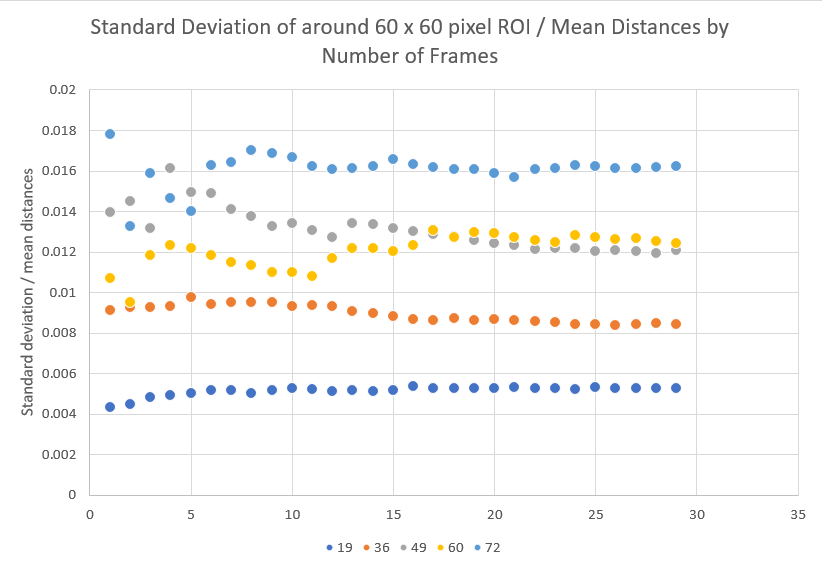
\includegraphics{images/d435_spatial_resolution.png}
\end{figure}

Here is the chart for sensor accuracy. The average errors by sensor are: 0.864 for the D435, 1.366 for the Azure Kinect, 1.739 for the D415, 2.446 for the Kinect Windows, and 2.489 for the Kinect XBOX.
\begin{figure}[h]
	\caption{Sensor accuracy by distance}
	\centering
	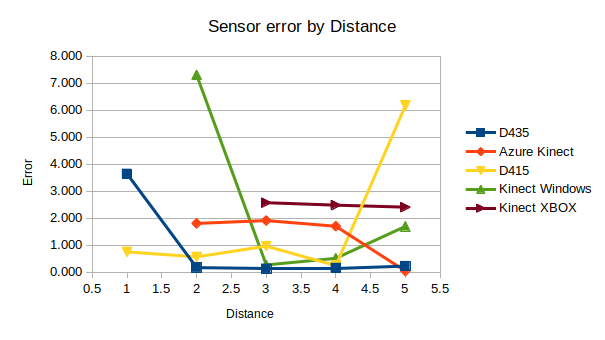
\includegraphics{images/sensor_accuracy.png}
\end{figure}

Here is the chart for temporal noise. Whereas the D435 scored the best, the D415 scored the best in this category. This is partly explained by the d435 being like the d415 except having its sensors more spread out. The winner in this category is the Kinect Azure with an average temporal noise of 0.07 percent, then comes the kinect for windows at 0.14, kinect 360 at 0.15, d415 at 0.22, and d435 and 3.99.
\begin{figure}[h]
	\caption{Sensor temporal noise by distance}
	\centering
	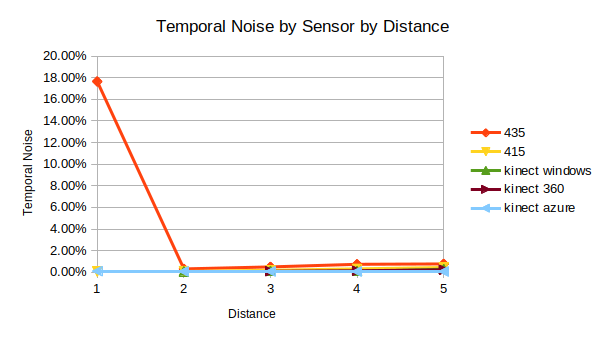
\includegraphics{images/temporal_noise.png}
\end{figure}

Here is the chart for fill rate. At first this metric may not seem that important but once you look at the actual depth images you can really see the difference between the sensors. If we exclude the kinect windows because it can't take data at 1 feet away and the kinect 360 which can't take data closer than 2 feet. The best sensors are d435 at 89.86 percent, d415 at 74.81, then Azure at 70.00. The Azure Kinect makes a very interesting design choice as the developers only keep pixels that the sensor is very confident in to maintain better accuracy. While the Kinect Windows and Kinect 360 trade this off by showing more valid pixels but have a reduced accuracy. With this judgement, it is even unclear whether the Azure kinect is even a better sensor in terms of specs as if one applied this same reduction in uncertain pixels in the kinect windows and kinect 360, those sensors may achieve comparable results.

\begin{figure}[h]
	\caption{Fill rate of sensor by distance}
	\centering
	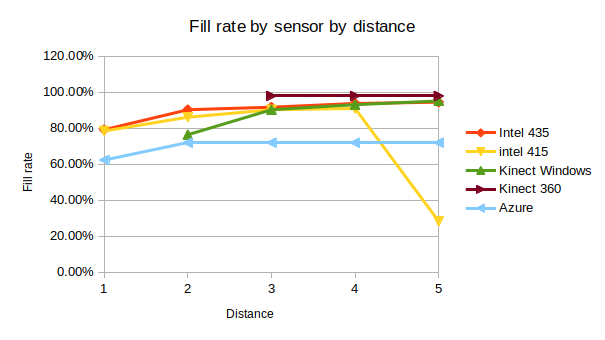
\includegraphics{images/fill_rate.png}
\end{figure}



\section{automated anthropometry results}
\section{gradient boosting body composition results}
\section{graph neural network body composition results}
\section{3d imaging testing results}
Results were as follows and are provided in the \hilight{figures}. 
\chapter{Conclusion}

This is going to be the chapter where I check the length of the page to make
sure the bottom margin works out all right.  I hope you don't mind long
annoying and useless paragraphs because you are sure to get a lot of them here!

\section{Widgets}

This is going to be the chapter where I check the length of the page
to make sure the bottom margin works out all right.  I hope you don't
mind long annoying and useless paragraphs because you are sure to get
a lot of them here!

\subsection{Sub-Widgets}

This is going to be the chapter where I check the length of the page
to make sure the bottom margin works out all right.  I hope you don't
mind long annoying and useless paragraphs because you are sure to get
a lot of them here!

\subsubsection{Sub-Sub-Widgets}

This is going to be the chapter where I check the length of the page
to make sure the bottom margin works out all right.  I hope you don't
mind long annoying and useless paragraphs because you are sure to get
a lot of them here!

\paragraph{Para-Widgets}

This is going to be the chapter where I check the length of the page
to make sure the bottom margin works out all right.  I hope you don't
mind long annoying and useless paragraphs because you are sure to get
a lot of them here!

\subparagraph{Sub-Para-Widgets}

This is going to be the chapter where I check the length of the page
to make sure the bottom margin works out all right.  I hope you don't
mind long annoying and useless paragraphs because you are sure to get
a lot of them here!

This is going to be the chapter where I check the length of the page
to make sure the bottom margin works out all right.  I hope you don't
mind long annoying and useless paragraphs because you are sure to get
a lot of them here!

This is going to be the chapter where I check the length of the page
to make sure the bottom margin works out all right.  I hope you don't
mind long annoying and useless paragraphs because you are sure to get
a lot of them here!

This is going to be the chapter where I check the length of the page
to make sure the bottom margin works out all right.  I hope you don't
mind long annoying and useless paragraphs because you are sure to get
a lot of them here!

This is going to be the chapter where I check the length of the page
to make sure the bottom margin works out all right.  I hope you don't
mind long annoying and useless paragraphs because you are sure to get
a lot of them here!

This is going to be the chapter where I check the length of the page
to make sure the bottom margin works out all right.  I hope you don't
mind long annoying and useless paragraphs because you are sure to get
a lot of them here!

This is going to be the chapter where I check the length of the page
to make sure the bottom margin works out all right.  I hope you don't
mind long annoying and useless paragraphs because you are sure to get
a lot of them here!

This is going to be the chapter where I check the length of the page
to make sure the bottom margin works out all right.  I hope you don't
mind long annoying and useless paragraphs because you are sure to get
a lot of them here!

This is going to be the chapter where I check the length of the page
to make sure the bottom margin works out all right.  I hope you don't
mind long annoying and useless paragraphs because you are sure to get
a lot of them here!

This is going to be the chapter where I check the length of the page
to make sure the bottom margin works out all right.  I hope you don't
mind long annoying and useless paragraphs because you are sure to get
a lot of them here!

This is going to be the chapter where I check the length of the page
to make sure the bottom margin works out all right.  I hope you don't
mind long annoying and useless paragraphs because you are sure to get
a lot of them here!

This is going to be the chapter where I check the length of the page
to make sure the bottom margin works out all right.  I hope you don't
mind long annoying and useless paragraphs because you are sure to get
a lot of them here!

This is going to be the chapter where I check the length of the page
to make sure the bottom margin works out all right.  I hope you don't
mind long annoying and useless paragraphs because you are sure to get
a lot of them here!

This is going to be the chapter where I check the length of the page
to make sure the bottom margin works out all right.  I hope you don't
mind long annoying and useless paragraphs because you are sure to get
a lot of them here!

This is going to be the chapter where I check the length of the page
to make sure the bottom margin works out all right.  I hope you don't
mind long annoying and useless paragraphs because you are sure to get
a lot of them here!

This is going to be the chapter where I check the length of the page
to make sure the bottom margin works out all right.  I hope you don't
mind long annoying and useless paragraphs because you are sure to get
a lot of them here!
